\chapter{Background \& Related Work}
\label{ch:background}

In this section we introduce the background necessary to understand the context of the project, and explore some related works which we utilise and build upon.

\section{Interfaces in Embedded Systems}

Interfacing between digital components is hard due to high speed and precision timing requirements, and is a problem continually explored by electronics engineers.

In consumer electronics the USB interface is very common, and devices include hardware USB controllers to handle the timing and signalling required to understand each other properly. On a desktop or laptop computer other interfaces such as SATA and PCIe can be found, which handle communication with internal peripherals such as hard drives and expansion cards like GPUs. Performance and timing accuracy is key in such applications, as consumers want their systems to be responsive and reliable. Dedicated interface hardware that is specialised for each protocol is standard in consumer systems, as it allows the CPU to continue to perform other tasks while I/O happens in the background. Communicaton between the CPU and I/O hardware usually happens via interrupts, shared memory, and/or DMA, all coordinated by system software usually within an OS kernel.

Microcontrollers and embedded systems are a similar story, except you're less likely to find a SATA interface on an MCU: interfaces such as SPI, UART, I\textsuperscript{2}C, PWM and CAN are more common, along with GPIO pins. These interfaces are more general-purpose, and designed for use with other electronic components rather than consumer hardware. They're also are a lot simpler than the likes of PCIe, and easy to implement into a small microcontroller fairly cheaply \cite{rp2040}.

This is fine for most cases, but the issue still remains that designers have a fixed and limited portfolio of hardware to choose from. It is often the case that a device does not include a specific interface that you need, or you have too many of one interface and not enough of another. Some more exotic peripherals may also include custom interfaces (to quote Raspbery Pi, `cursed serial device found on AliExpress`) which are not supported in any of the existing hardware.

As an example, Espressif's ESP32 is one of the most popular microcontrollers on the market at the moment, due to a combination of it's low cost and WiFi \& Bluetooth capabilities. In terms of digital I/O hardware, the device has 3 UART interfaces, two I\textsuperscript{2}C buses, two I\textsuperscript{2}S buses, three SPIs, a PWM controller, a TWAI/CAN (Two Wire Automotive Interface) controller, an SDIO/SPI slave controller, and an SD/SDIO/MMC host controller \cite{esp32}. This is a broad complement of I/O hardware that is representative of most devices on the market, but if a designer did want to connect more than three SPI devices, or a peripheral that doesn't support one of the aforementioned protocols, then they are left in a difficult situation.

One solution to this is to use the processing system of a microcontroller to read/write to the GPIO pins at high speeds to implement the required signalling such that the external hardware can understand the data. This is a technique known as `bit-banging', and is very hard because CPUs are not designed for this, and usually cannot meet the precise timing requirements of external devices. Programmers often carefully craft very tight loops in assembly in the hope that the CPU will execute their instructions on the exact cycle that they want them to, but with the increasing complexity of modern CPUs and the advent of out-of-order architectures, this is increasingly rare. CPU time is also precious in embedded systems, and bit-banging consumes lots of power and processor cycles.

The proper solution to custom interface requirements is custom hardware, but this can be very expensive. Designing a custom microprocessor and getting it manufactured can cost hundreds of thousands if not millions, and is not practical to do in small quantities. The field-programmable gate array, or FPGA is another solution: an array of configurable logic cells with a programmable interconnect that can be programmed to implement arbitrary logic circuits. FPGAs are very flexible, and capable of high I/O throughput with absolute precision and control. However, they can be very expensive, an order of magnitude more than most low-cost microcontrollers. FPGAs also present a very unique programming model which may be unfamiliar to most software engineers, making them hard to work with.

Embedded systems including FPGAs are not uncommon for high-performance or highly custom applications: Xilinx's Zynq-7000 system-on-chips (SoCs) combine programmable logic with a two ARM Cortex-A9 CPU cores as shown in figure \ref{fig:zynq}. The SoC also includes standard external interfaces such as I2C and SPI, but can be programmed to add additional interfaces through the programmable logic subsystem.

\begin{figure}[H]
    \centering
    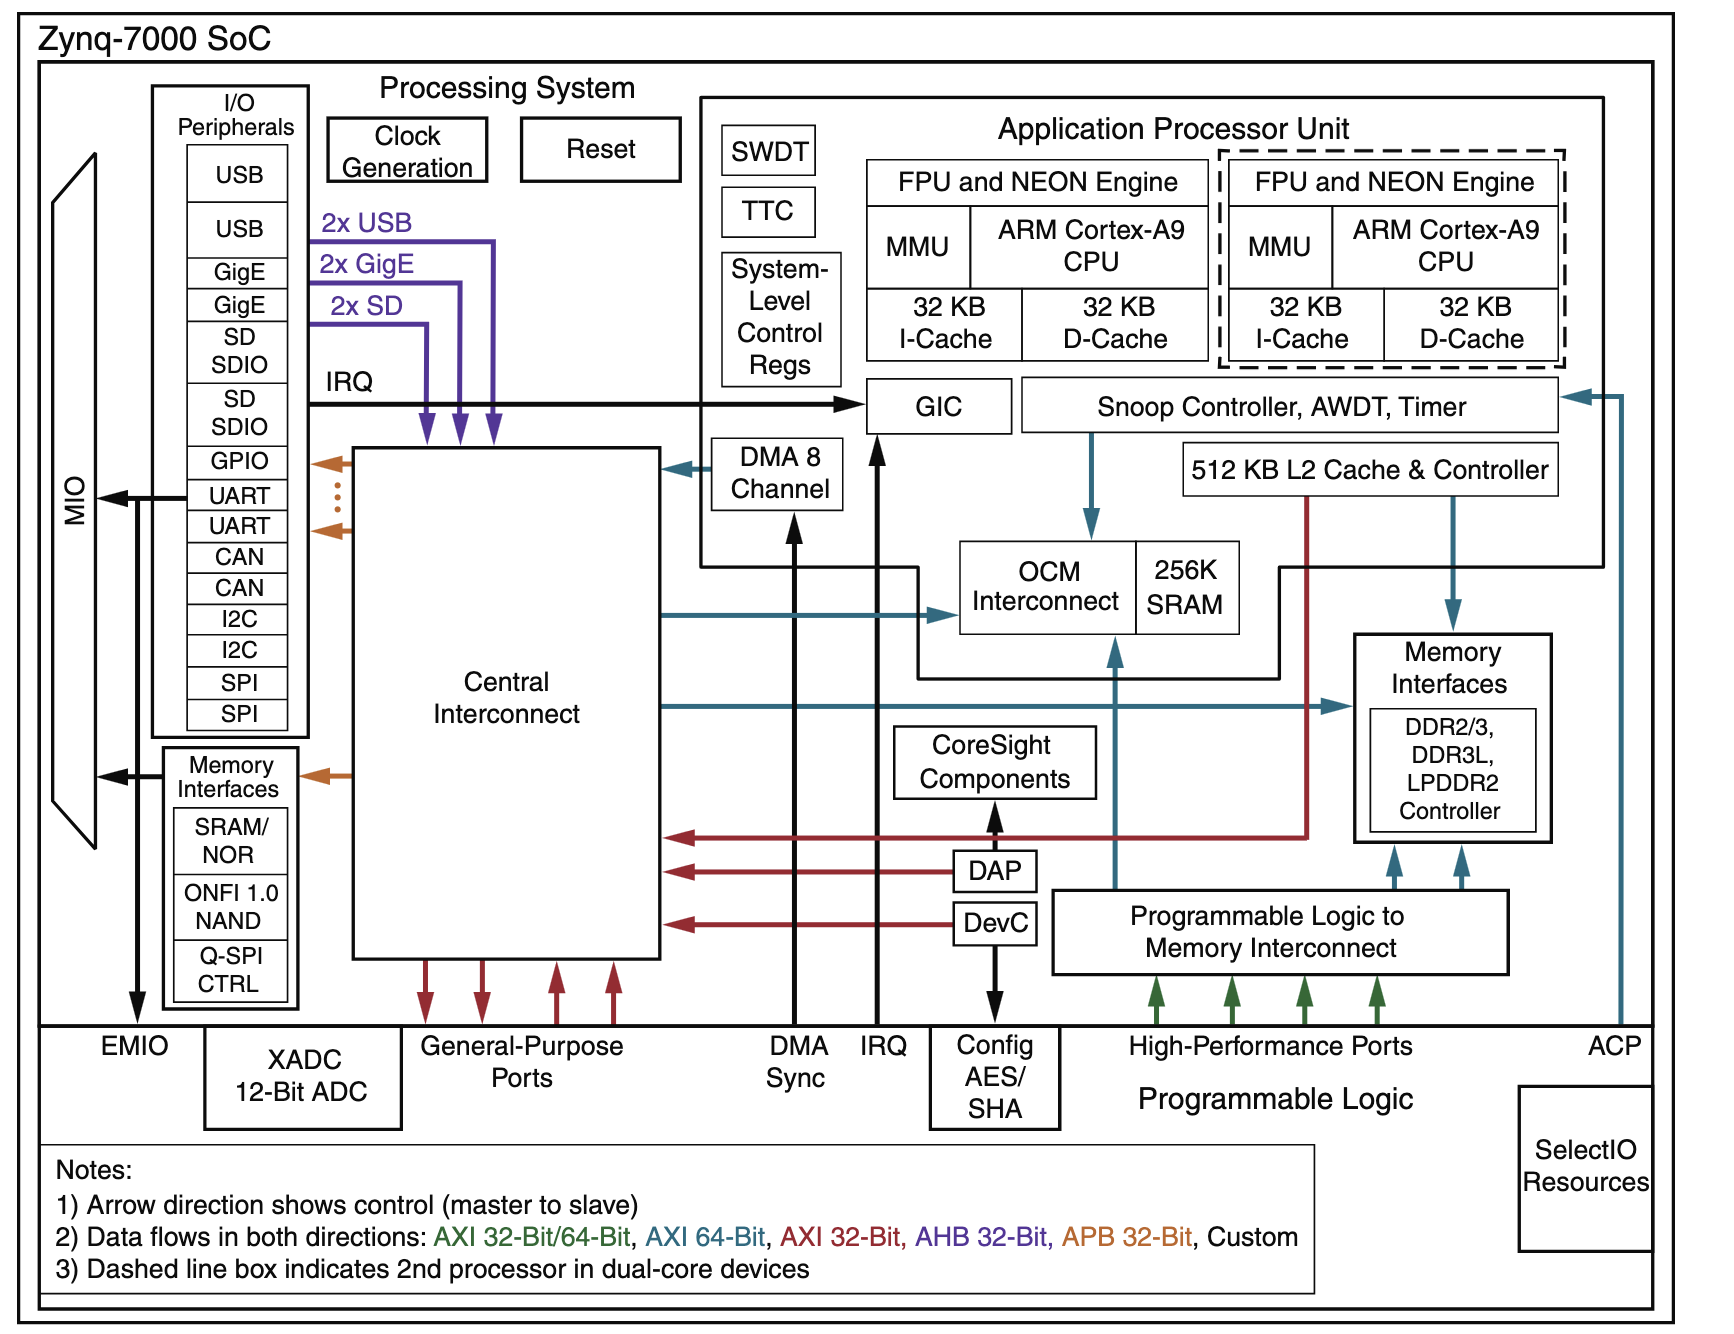
\includegraphics[width=0.85\textwidth]{../img/zynq.png}
    \caption{Block diagram of Xilinx's Zynq-7000 Architecture \citep{zynq}}
    \label{fig:zynq}
\end{figure}


\section{The RP2040 and PIO}
Raspberry Pi acknowledge all these issues in their introduction to the RP2040's PIO in their documentation, pitching it as a way to add additional hardware interfaces to a device without the drawbacks of bit-banging or programmable logic. PIO is fixed-function hardware included in the RP2040 with a similar power draw and chip area utilisation to a typical hardware interface, built to operate with cycle-accuracy and determinism at up to 48MHz (the system clock speed), allowing it to meet the timing requirements necessary for many high-speed serial interfaces.

Figure \ref{fig:pio-sm} gives an overview of one of the PIO state machines. Included in each one are two 32-bit shift registers, two 32-bit scratch registers, a clock divider, flexible GPIO pin mapping, and 2 4x32-bit FIFOs connected to the system bus. Each PIO block includes 4 state machines, each capable of executing independently. The architecture is designed to perform a small set of operations, primarily setting/clearing GPIO pins, and moving data to/from the processor (optionally using the DMA subsystem) \cite{rp2040}.

\begin{figure}[H]
    \centering
    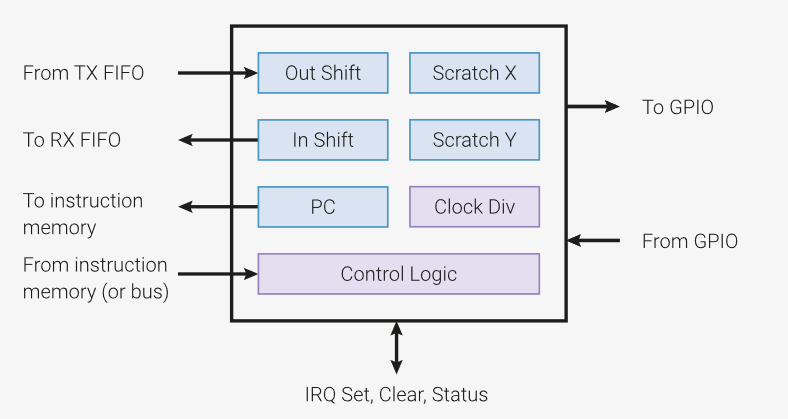
\includegraphics[width=0.7\textwidth]{../img/rp2040-state-machine.png}
    \caption{An overview of a PIO State Machine \citep{rp2040}}
    \label{fig:pio-sm}
\end{figure}

The flexibility and power of the PIO blocks allow them to be programmed to implement common interfaces such as UART and SPI, more complex interfaces such as DVI and SDIO, and even custom interfaces to enable tight integration with other external hardware bespoke embedded systems.

\subsection{PIO Assembly Language}
The RP2040 PIO is programmable via a small assembly-like DSL called pioasm. It contains only 9 instructions, each executed within a single clock cycle. The instruction set is very dense: the PIO is capable of sampling a GPIO pin, toggling an output clock, and pushing a data word to the system all with a single instruction. An small example program is shown in Listing \ref{lst:sqwave} that outputs a square wave on a single GPIO pin.

\begin{listing}[b]
    \vspace{0.5cm}
    \begin{minted}{asm}
.program squarewave
set pindirs, 1   ; Set pin to output
again:
set pins, 1 [1]  ; Drive pin high then delay for one cycle
set pins, 0      ; Drive pin low
jmp again        ; Set PC to label `again`
    \end{minted}
    \caption{PIO Assembly to output a square wave \citep{rp2040}}
    \label{lst:sqwave}
\end{listing}

Listing \ref{lst:sqwave} uses only 2 of the 9 instructions: \mintinline{text}|set| to drive GPIO pins, and \mintinline{text}|jmp| to implement a loop. More details on pioasm is given in Chapter \ref{ch:design} as part of our design discussion.

\section{I/O Coprocessors}
The idea of offloading I/O to a coprocessor is not novel. We explore two other devices which include subsystems that are designed for I/O.
\subsection{Time Processor Unit}

The Time Processor Unit (TPU) is a coprocessing subsystem found in some older Motorola microcontrollers \cite{tpu}, built upon by the Enhanced TPU (eTPU) in NXP Semiconductor's MCF523x family of microcontrollers build on the ColdFire architecture \cite{mfcdatasheet}.

The eTPU is a real-time microprocessed system, designed to run microengine code on a built-in RISC processor to respond to events triggered by either internal timers, interrupts, or I/O transitions. Each eTPU engine consists of 32 channels, each with an input and output, and containing logic to listen for up to 4 events. Channels can be independently configured to perform functions such as output generation, input capture, or a combination of the two.

Communication between the eTPU and host CPU happens via a shared RAM, which can be used for data transfer between the two, and as storage for eTPU microcode programs. The CPU configures the eTPU by writing to the relevant configuration registers within the system's address space, and can configure each channel mode and priority independently \cite{etpu}.

The event-driven architecture differs from that of the RP2040's PIO, in that timing is decoupled from the microcode execution: code is executed in response to an event, rather than the timing being built in to the execution of the code. However, the guarantees provided by the hardware around event response latency and the nature of microcode execution within the TPU means it can meet the timing requirements necessary for interfaces such as UART.

\subsection{ESP-32 Ultra Low Power Coprocessor}

The ESP-32 contains an ultra-low power coprocessor (ULP) that can remain powered on when the rest of the SoC is in deep sleep mode. The ULP is a finite state machine can execute a program from it's own memory that is capable of accessing peripheral devices and internal sensors, and communicating via I\textsuperscript{2}C. It can wake the CPU and send interrupts to the host system, as well as control it's own sleep state. It can communicate with the rest of the SoC via a shared memory that can be read/written by the ULP while the rest of the SoC is in deep sleep. It can be started directly by software on the host system, or by a hardware timer triggered periodically.

Unlike PIO and the eTPU, the ULP is not designed to implement arbitrary I/O protocols, instead acting as a co-processor that has access to only I\textsuperscript{2}C, ADC and GPIO interface hardware. Instead, it's purpose is to offload I/O functions from the CPU to save power. Given the ESP32 positioning itself as an IoT microcontroller, this makes sense, as IoT devices often want to consume as little power as possible.\cite{esp32}

Despite this, the idea of an I/O-focused coprocessor designed to operate in ultra-low power states is powerful. IoT devices often operate on tightly contstrained power budgets, and as battery-powered embedded systems become more prevalent in applications such as wearables and wireless devices, the need for I/O at low power is evident.

\section{RISC-V}

RISC-V is an open standard instruction set architecture. Originally developed at the University of California, Berkely to support computer architecture research and education, it has grown into an industry standard and is being used in commercial devices. RISC-V was designed explicitly to be an open standard ISA, but also to be `a \textit{real} ISA'\cite{riscv_design}, such that it would be suitable for hardware implementation in an FPGA or ASIC. It was also designed to be highly flexible and extensible, a factor showcased by it's many extension standards \cite{riscv_spec}.

supported in software tools like linux

commercial devices like sifive and other examples

It is for these reasons we explore RISC-V for this project: it's open source nature means it is free for us to use and experiment with, and many well-supported open source implementations are available. It's flexibility also means it is possible to easily and closely integrate external peripherals.


\subsection{Rocket Chip}

Rocket Chip is one such implementation.

- open course RISC-V SoC generator framework
- has been taped out before
- what does it include
- rocket core and BOOM

\section{Chisel}
Rocket chip is written in chisel, a novel HDL eDSL scala
leverages it to provide parametriseability and flexibility
- issues with current HDLs
- how Chisel fixes these
- also provides Firrtl and chiseltest and treadle

\section{Rust for Embedded Systems}



\section{FPGAs}
FPGAs are an implementation detail of this project and are introduced as such.
- what is it (quote xilinx)
- why is it useful (rapi)
- why would we usually use an ASIC for something like this
